\documentclass{beamer}

\usetheme[progressbar=frametitle]{metropolis}
\usepackage{appendixnumberbeamer}
\usepackage{booktabs}
\usepackage{amsmath}
\usepackage{amssymb}
\usepackage{tcolorbox}
\usepackage{tikz}

\definecolor{metropolisblue}{RGB}{39, 59, 94}



% Begin document
\begin{document}

% Title page
\title{Sampling Methods}
\author{Nipun Batra}
\date{\today}
\institute{IIT Gandhinagar}
\maketitle

\begin{frame}{Topics}
    %TOC with enumerated items
    \setbeamertemplate{section in toc}[sections numbered]
    \tableofcontents

\end{frame}

\section{Markov Chains}
\begin{frame}
    \url{https://nipunbatra.github.io/hmm/}
\end{frame}

\begin{frame}{Global Optimization}
    Notebook: mcmc=optimization.ipynb
    
\end{frame}


\begin{section}{Importance Sampling}
    \begin{frame}{General Form}
        In rejection sampling, we saw that due to less acceptance probability, a lot of samples were wasted leading to more time and higher complexity to approximate a distribution.

        Computing $p(x), q(x)$ thus seems wasteful. Let us rewrite the equation as:
        \begin{align*}
            \phi &= \int f(x)p(x)dx = \int f(x)\frac{p(x)}{q(x)}q(x)dx \\
            &\sim \frac{1}{N} \sum_{i=1}^Nf(x_i)\frac{p(x_i)}{q(x_i)} = \frac{1}{N} \sum_{i=1}^Nf(x_i)w_i 
        \end{align*}
        Here, $x_i\sim q(x)$. $w_i$ is known as the importance(weight) of sample i. 
    \end{frame}

    \begin{frame}
        However the normalization constant $Z$ is generally not known to us. Thus writing: 
        \begin{equation}
            p(x) = \frac{\Tilde{p}(x)}{Z}
        \end{equation}
        Now inserting this in earlier equations, we get:
        \begin{align*}
            \phi &=\frac{1}{Z} \int f(x)\Tilde{p}(x)dx = \frac{1}{Z}\int f(x)\frac{\Tilde{p}(x)}{q(x)}q(x)dx \\
            &\sim \frac{1}{NZ} \sum_{i=1}^Nf(x_i)\frac{\Tilde{p}(x_i)}{q(x_i)} = \frac{1}{NZ} \sum_{i=1}^Nf(x_i)w_i 
        \end{align*}
        We know that:
        \begin{align*}
            Z &= \int_{\infty}^{\infty} \Tilde{p}(x)dx = \int_{\infty}^{\infty}\frac{\Tilde{p}(x)}{q(x)}q(x)dx \\
            &= \frac{1}{N}\sum_{i=1}^N w_i
        \end{align*}
    \end{frame}

    \begin{frame}
        Substuting this value of $Z$ in the equation above, we get:
        \begin{align*}
            \phi &= \frac{1}{N}\sum_{i=1}^N f(x_i)w_i = \frac{\sum_{i=1}^N f(x_i)w_i}{\sum_{i=1}^N w_i} \\
            &= \sum_{i=1}^N f(x_i)W_i
        \end{align*}
        Here $W_i = \frac{w_i}{\sum_{i=1}^N w_i}$ are the normalized weights.
    \end{frame}

    \begin{frame}{Limitations}
        \begin{itemize}
            \item Recall that Var $\hat{\phi} = \frac{var(f)}{N}$. Importance sampling replaces $var(f)$ with $var(f\frac{p}{q})$. At positions where $p>>>q$, the weight can tend to $\infty$!
        \end{itemize}
        \begin{figure}
                \centering
                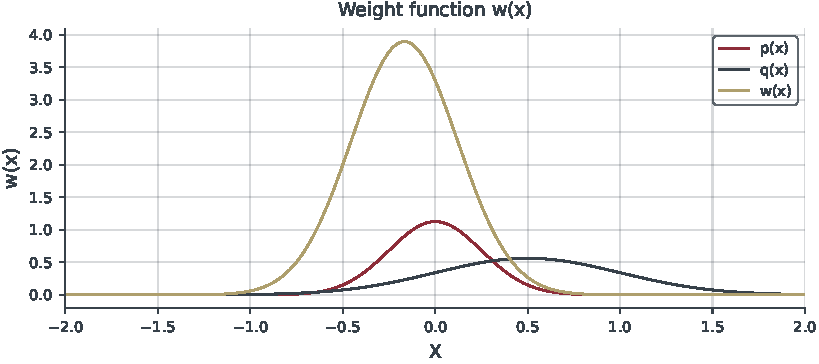
\includegraphics[scale=0.8]{../figures/importance_sampling_weight_function.pdf}
        \end{figure}
    \end{frame}
\end{section}

\begin{section}{Gibbs Sampling}
    \begin{frame}{General Form}
        Suppose we wish to sample $\theta_1, \theta_2 \sim p(\theta_1, \theta_2)$, but cannot use:\\
        \begin{itemize}
            \item direct simulation
            \item accept-reject method
            \item Metropolis-Hasting
        \end{itemize}
        But we can sample using the conditionals i.e.:\\
        \begin{itemize}
            \item $p(\theta_1|\theta_2)$ and
            \item $p(\theta_2|\theta_1)$,
        \end{itemize}
        then we can use Gibbs sampling.
    \end{frame}
    
    \begin{frame}
        Suppose $\theta_1, \theta_2 \sim p(\theta_1, \theta_2)$ and we can sample from $p(\theta_1, \theta_2)$. We begin with an initial value $(\theta_1^{0}, \theta_2^{0})$, the workflow for Gibbs algorithm is:\\
        1. sample $\theta_1^j \sim p(\theta_1|\theta_2^{j-1})$ and then\\
        2. sample $\theta_2^j \sim p(\theta_2|\theta_1^j)$.\\
        One thing to note here is that the sequence in which the theta's are sampled are not independent!    
    \end{frame}

    \begin{frame}{Bivariate Normal Example}
        Suppose \\
        $\theta \sim N_2(0,\Sigma)$ and $\Sigma = $
        $ \begin{matrix}
        1 & \rho \\
        \rho & 1  
        \end{matrix} $
    
    Then, we have:\\
    $\theta_1|\theta_2 \sim N(\rho\theta_2,[1-\rho^2])$

    $\theta_2|\theta_1 \sim N(\rho\theta_1,[1-\rho^2])$
    are the conditional distributions.
    The Gibbs sampling proceeds as follows:\\
    \begin{table}[]
        \centering
        \begin{tabular}{c c c}
           Iteration & Sample $\theta_1$ & Sample $\theta_2$\\
           \hline
           1  &  $\theta_1\sim N(\rho\theta_2^0, [1-\rho^2])$ &  $\theta_2\sim N(\rho\theta_1^1, [1-\rho^2])$\\
           & . & \\
           & . & \\
           $k$  &  $\theta_1\sim N(\rho\theta_2^{k-1}, [1-\rho^2])$ &  $\theta_2\sim N(\rho\theta_1^k, [1-\rho^2])$
             
        \end{tabular}
    \end{table}
    \end{frame}

    \begin{frame}
        \begin{figure}
                \centering
                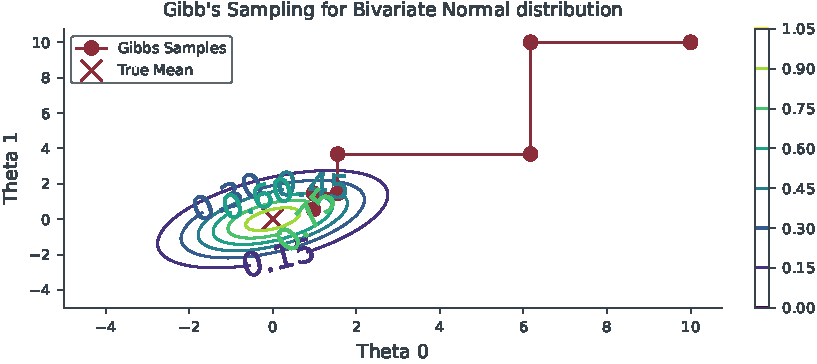
\includegraphics[scale=0.8]{../figures/gibbs_sampling_bivariate_normal.pdf}
            \end{figure}
    \end{frame}

    \begin{frame}{Multivariate case}
        Suppose $\theta = (\theta_1, \theta_2, \ldots, \theta_K)$, the Gibbs workflow is as follows:\\
        $\theta_1^j = p(\theta_1|\theta_2^{j-1}, \ldots, \theta_K^{j-1})$\\
        $\theta_2^j = p(\theta_2|\theta_1^{j}, \theta_3^{j-1}, \ldots, \theta_K^{j-1})$\\
        .\\
        .\\
        $\theta_k^j = p(\theta_k|\theta_1^{j}, \ldots, \theta_{k-1}^j, \theta_{k+1}^{j-1}, \ldots, \theta_K^{j-1})$\\
        .\\
        .\\
        $\theta_K^j = p(\theta_K|\theta_1^{j}, \ldots, \theta_{K-1}^{j})$\\
        The distributions above are call the full conditional distributions.
    \end{frame}

    \begin{frame}{Advantages}
        Gibbs sampling can be used to draw samples from $p(\theta)$ when:\\
        \begin{itemize}
            \item Other methods don't work quite well in higher dimensions.
            \item Draw samples from the full conditional distributions is easy, $p(\theta_k|\theta_{-k}).$
        \end{itemize}
    \end{frame}
\end{section}

\begin{section}{Markov Chain Monte Carlo}
    \begin{frame}{Limitations of basic sampling methods}
        \begin{itemize}
            \item \textit{Transformation based methods}: Usually limited to drawing from standard distributions.
            \item \textit{Rejection and Importance sampling}: Require selection of good proposal distirbutions.
        \end{itemize}
        In high dimensions, usually most of the density $p(x)$ is concentrated within a tiny subspace of $x$. Moreover, those subspaces are difficult to be known a priori.

        A solution to these are MCMC methods.
    \end{frame}

    \begin{frame}{Markov Chain}
        \begin{itemize}
            \item \textbf{Markov Chain}: A joint distribution $p(X)$ over a sequence of random variables $X = \{X_1, X_2, \ldots, X_n\}$ is said to have the Markov property if 
            $$
            p(X_i|X_1, \ldots, X_{i-1}) = p(X_i|X_{i-1}) 
            $$
            The sequence is then called a Markov chain.
            \item The idea is that the estimates contain information about the shape of the target distribution $p$.
        \end{itemize}
    \end{frame}

    \begin{frame}{Metropolis Hastings}
        \begin{itemize}
            \item The basic idea is propose to move to a new state $x_{i+1}$ from the current state $x_i$ with probability $q(x_{i+1}|x_i)$, where $q$ is called the proposal distribution and our target density of interest is $p (= \frac{1}{Z} \tilde{p})$.
            \item The new state is accepted with probability $\alpha(x_i, x_{i+1})$.
            \begin{itemize}
                \item If $p(x_{i+1}| x_i) = p(x_i| x_{i+1})$, then $\alpha(x_i, x_{i+1}) = \min (1, \frac{p(x_{i+1})}{p(x_i)})$.
                \item If $p(x_{i+1}| x_i) \neq p(x_i| x_{i+1})$, then $\alpha(x_i, x_{i+1}) = \min (1, \frac{p(x_{i+1})q(x_i|x_{i+1})}{p(x_i)q(x_{i+1}|x_i)}) = \min (1, \frac{\tilde{p}(x_{i+1})q(x_i|x_{i+1})}{\tilde{p}(x_i)q(x_{i+1}|x_i)})$
            \end{itemize}
            \item Evaluating $\alpha$, we only need to know the target distribution up to a constant of proportionality or without normalization constant.
        \end{itemize}
    \end{frame}

    \begin{frame}{Algorithm: Metropolis Hastings}
        \begin{enumerate}
            \item Initialize $x_0$.
            \item for $i = 1, \ldots, N$ do:
            \item \quad Sample $x^* \sim q(x^*|x_{i-1})$.
            \item \quad Compute $\alpha = \min (1, \frac{\tilde{p}(x^*)q(x_{i-1}|x^*)}{\tilde{p}(x_{i-1})q(x^*|x_{i-1})})$
            \item \quad Sample $u \sim \mathcal{U}(0, 1)$
            \item \quad if $u \leq \alpha$:
            
            \quad \quad $x_i = x^*$
            
            \quad else:
            
            \quad \quad $x_i = x_{i-1}$
        \end{enumerate}
    \end{frame}

    \begin{frame}{Pop Quiz}
        How do we choose the initial state $x_0$?
        \pause
        \begin{enumerate}
            \item Start the Markov Chain at an initial $x_0$.
            \item Using the proposal $q(x|x_i)$, run the chain long enough, say $N_1$ steps.
            \item Discard the first $N_1 - 1$ samples (called 'burn-in' samples).
            \item Treat $x_{N_1}$ as first sample from $p(x)$.
        \end{enumerate}
    \end{frame}

    \begin{frame}{MCMC demo}
        
        \url{https://chi-feng.github.io/mcmc-demo/app.html}
    \end{frame}
\end{section}

\end{document}